\chapter{Handbook}
\label{chap:handbook}
 
\section{Chapters}

\subsection{Adding a new chapter}

To add a new chapter, follow the next steps:

\begin{enumerate}
  \item Create a new file in the \verb|chapters| folder and name this file using \verb|dash-case|, meaning that every word in the file name is\\\verb|lowecase-and-separated-with-dashes|.
  \item Go to the \verb|main.tex| file and find the "\verb|% CHAPTERS|" comment.\\Check how other chapters have been included as an example.
  \item Include your new chapter as follows:
  \begin{lstlisting}
    \include{chapters/you-new-chapter}\end{lstlisting}
  \item Go to your chapter file and paste the following basic code:
  \begin{lstlisting}
    \chapter{New Chapter}

    % use to be referenced
    \label{chap:<chapterLabel>}
 
    \section{First Section}
    
    Your section content here.
    
    \section{Second Section}
    
    Your section content here.
    
    \subsection{First Subsection}

    Your subsection content here.

    \subsubsection{First Subsubsection}

    Your subsubsection content here.
    
    \section*{Unnumbered Section}

    Your unnumbered section content here.\end{lstlisting}
  \item Your can find a similar code in the \verb|chapters/example.tex| file. It might be easier for you to copy it from there. Got to the chapter \ref{chap:example} (Example) to see how it looks like.
\end{enumerate}

\subsection{Reference chapters}

You can dynamically reference a chapter as in \textbf{chapter \ref{chap:handbook}} (this chapter). References will be properly updated if something change with the chapter page.

\begin{lstlisting}
  % Reference a chapter
  \ref{fig:<chapterLabel>}
\end{lstlisting}

\section{Text and Paragraphs}

\subsection{New line}

Use \verb|\\| or \verb|\newline| to create a new line - equivalent to \verb|Shift+Enter|. Care should be taken that multiple \verb|new lines| are not used to "simulate" paragraphs with larger spacing between them.

\begin{lstlisting}
  This is one line.
  \\
  This is another line.
  \\
  This is one more line.
\end{lstlisting}

\subsection{New paragraph}

To start a new paragraph you can just leave one line space from one text from the other in your \textbf{editor}:

\begin{lstlisting}
  % These two lines are in the same paragraph
  This is one sentence. This is another sentence.
  This is no more sentence.

  % These two lines are in two different paragraphs
  This is one paragraph.

  This is another paragraph.
\end{lstlisting}

\bigskip

You can also be explicit on creating a new paragraph using \verb|\par|:

\begin{lstlisting}
  % These two lines are in two different paragraphs
  This is one paragraph.\par This is another paragraph.
\end{lstlisting}

\subsection{Alignment}

\begin{center}
  This text is an example of Center Alignment (\verb|center|) using the center environment. You can also use \verb|flushleft| (left alignment) and \verb|flushright| (right alignment).
\end{center}

\begin{lstlisting}
  \begin{center}
    This text is an example of Center Alignment.
  \end{center}
\end{lstlisting}

\subsection{Lists}

\subsubsection{Unordered}

\begin{itemize}
  \item Lorem ipsum dolor sit amet, consectetur adipiscing elit. In finibus felis nunc, et sagittis velit consectetur eget.
  \item Lorem ipsum dolor sit amet, consectetur adipiscing elit. In finibus felis nunc, et sagittis velit consectetur eget.
\end{itemize}

\begin{lstlisting}
  \begin{itemize}
    \item Your item 1.
    \item Your item 2.
  \end{itemize}
\end{lstlisting}

\subsubsection{Ordered}

\begin{enumerate}
  \item Lorem ipsum dolor sit amet, consectetur adipiscing elit. In finibus felis nunc, et sagittis velit consectetur eget.
  \item Lorem ipsum dolor sit amet, consectetur adipiscing elit. In finibus felis nunc, et sagittis velit consectetur eget.
\end{enumerate}

\begin{lstlisting}
  \begin{enumerate}
    \item Your item 1.
    \item Your item 2.
  \end{enumerate}
\end{lstlisting}

\section{Font Format}
 
Some of the \textbf{greatest} discoveries in \underline{science} were made by \textbf{\textit{accident}}. This is an \emph{emphasized} word inside normal text. \textit{And this is an \emph{emphasized} word inside an italicized text.}

\subsection{Bold}
\begin{lstlisting}
  \textbf{<your text>}
\end{lstlisting}

\subsection{Underline}
\begin{lstlisting}
  \underline{<your text>}
\end{lstlisting}

\subsection{Italic}
\begin{lstlisting}
  \textit{<your text>}
\end{lstlisting}

\subsection{Emphasis}
\begin{lstlisting}
  \emph{<your text>}
\end{lstlisting}

\section{References and Citations}

\subsection{Quotation}

\subsubsection{Display quotation}

Lorem ipsum dolor sit amet, consectetur adipiscing elit:
 
\begin{displayquote}
  \blindtext
\end{displayquote}

\begin{lstlisting}
  \begin{displayquote}
    <your text>
  \end{displayquote}
\end{lstlisting}

\subsubsection{In-line quotation}

Suspendisse nec pellentesque nunc \textquote{sed massa diam, gravida ut est sit amet, molestie viverra nunc}, lorem ipsum dolor sit amet, consectetur adipiscing elit.

\begin{lstlisting}
  \textquote{<your text>}
\end{lstlisting}

\subsection{Bibliography management}

Bibliographic references are usually kept in a bibliography file whose extension is \verb|.bib|. This file consists of a list of records and fields. Each bibliography record holds relevant information for a single entry.

\subsubsection{Example}

\begin{lstlisting}
  @book{latexcompanion,
      author    = "Michel Goossens and Frank Mittelbach and Alexander Samarin",
      title     = "The \LaTeX\ Companion",
      year      = "1993",
      publisher = "Addison-Wesley",
      address   = "Reading, Massachusetts"
  }
\end{lstlisting}

\subsection{Bibliography file generation}

Normally, you don't have to generate the bibliography file by yourself, you can use a reference manager such as \href{https://www.mendeley.com}{Mendeley} to do that, \href{https://blog.mendeley.com/2012/03/24/how-to-series-generate-bibtex-files-for-your-collections-for-use-in-latex-part-3-of-12/}{as explained in this blog article}.

Furthermore, if you are using a modern latex editor, such as \href{https://www.overleaf.com}{Overleaf}, you might be able to direclty synchronize your bibliography file with your renference manager tool. Check the following \href{https://www.overleaf.com/blog/639-tip-of-the-week-overleaf-and-reference-managers}{blog article} to learn more.

\subsection{Bibliography style}

This template uses the APA Style for references and citations. If you want change it, go to the \verb|main.tex| file of this template, find the\\\verb|\bibliographystyle{apalike}| line, and change the \verb|apalike| parameter for any of the \href{https://www.overleaf.com/learn/latex/Bibtex_bibliography_styles}{supported styles} by Bibtex.

\subsection{Citation}

This document is an example of \texttt{thebibliography} environment using  in bibliography management. Three items are cited: \textit{The \LaTeX\ Companion} book \cite{latexcompanion}, the Einstein journal paper \cite{einstein}, and the Donald Knuth's website \cite[p.150]{knuthwebsite}. The \LaTeX\ related items are \cite{latexcompanion,knuthwebsite}.

\begin{lstlisting}
  % One reference
  \cite{<ref-id>}

  % One reference with additional info (like page)
  \cite[<additional info>]{<ref-id>}

  % Two or more references
  \cite{<ref-id-1>,<ref-id-2>}
\end{lstlisting}

\section{Images and Figures}

\subsection{Baseline images}

Lorem ipsum dolor sit amet, consectetur adipiscing elit. Suspendisse nec pellentesque nunc. Sed massa diam, gravida ut est sit amet, molestie viverra nunc. Nam id ex ut tortor viverra auctor. 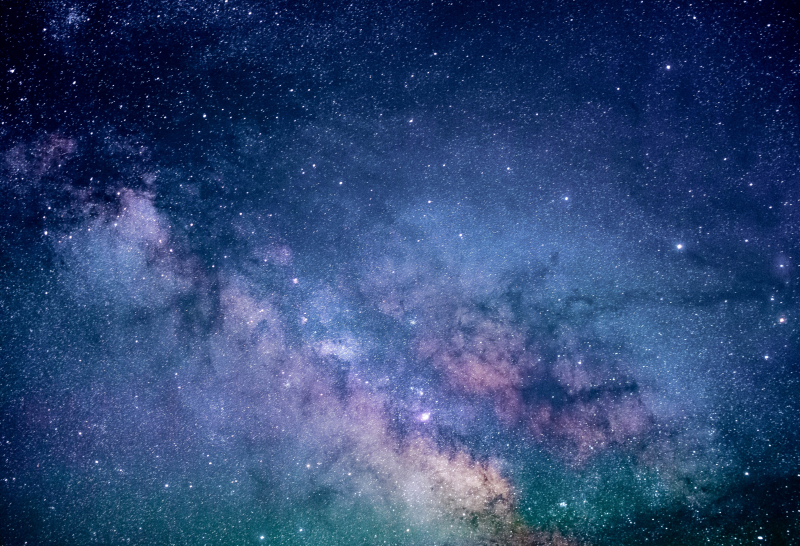
\includegraphics[height=\baselineskip]{image-1} Lorem ipsum dolor sit amet, consectetur adipiscing elit. Suspendisse nec pellentesque nunc. Sed massa diam, gravida ut est sit amet, molestie viverra nunc. Nam id ex ut tortor viverra auctor. 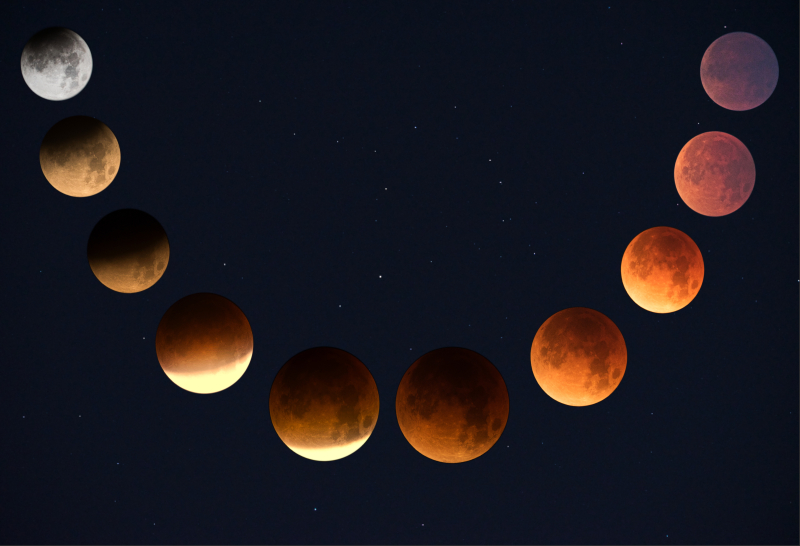
\includegraphics[height=\baselineskip]{image-2}.

\begin{lstlisting}
  \includegraphics[height=\baselineskip]{<file-name>}
\end{lstlisting}

\clearpage
\subsection{Full width image}

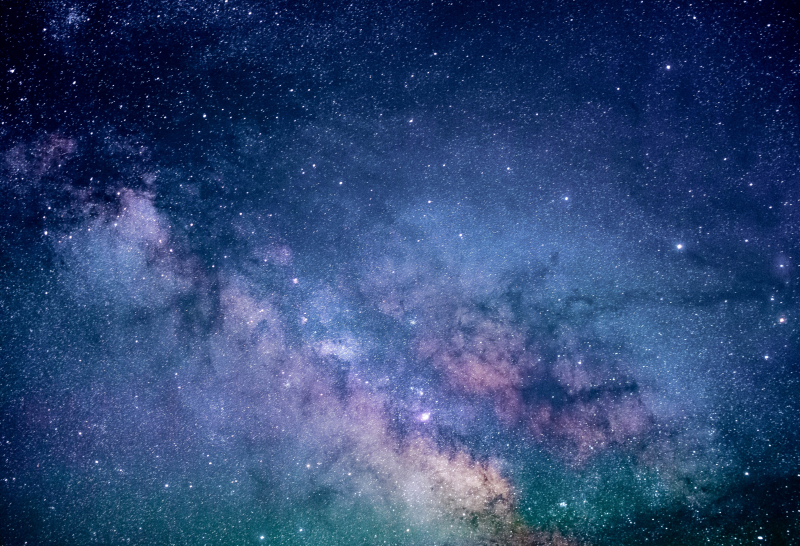
\includegraphics[width=\linewidth]{image-1}

\begin{lstlisting}
  \includegraphics[width=\linewidth]{<file-name>}
\end{lstlisting}

\clearpage
\subsection{Image with specific height}

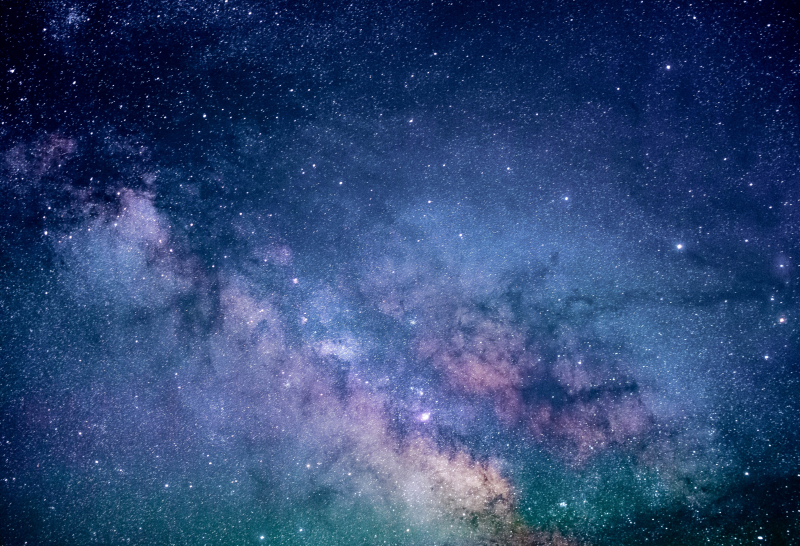
\includegraphics[height=3cm]{image-1}

\begin{lstlisting}
  \includegraphics[height=3cm]{<file-name>}
\end{lstlisting}

\clearpage
\subsection{Grid of images}

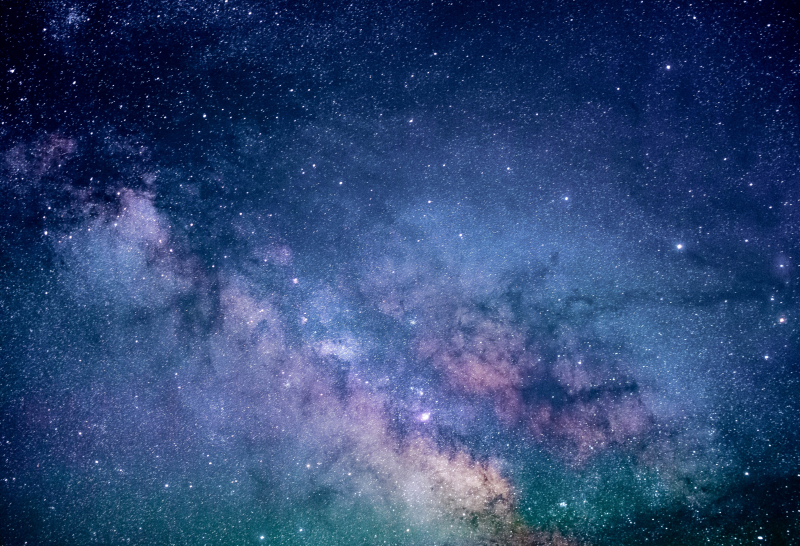
\includegraphics[width=0.3\linewidth]{image-1}
\quad
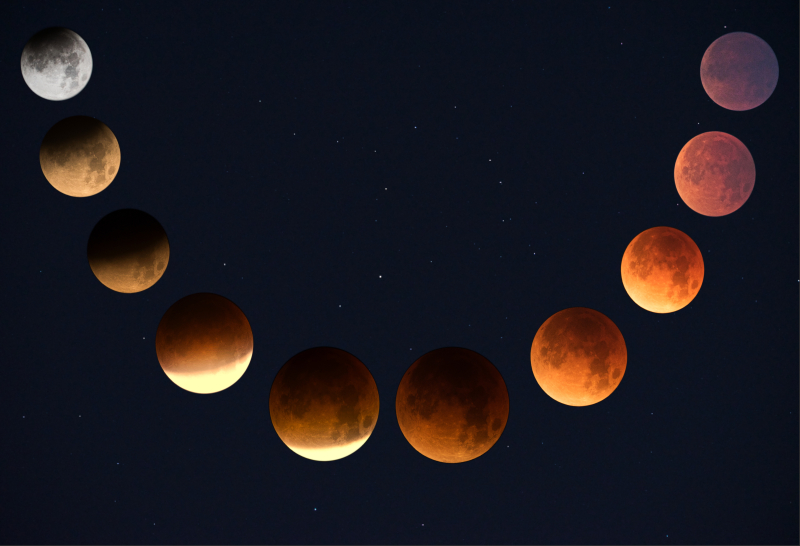
\includegraphics[width=0.3\linewidth]{image-2}
\quad
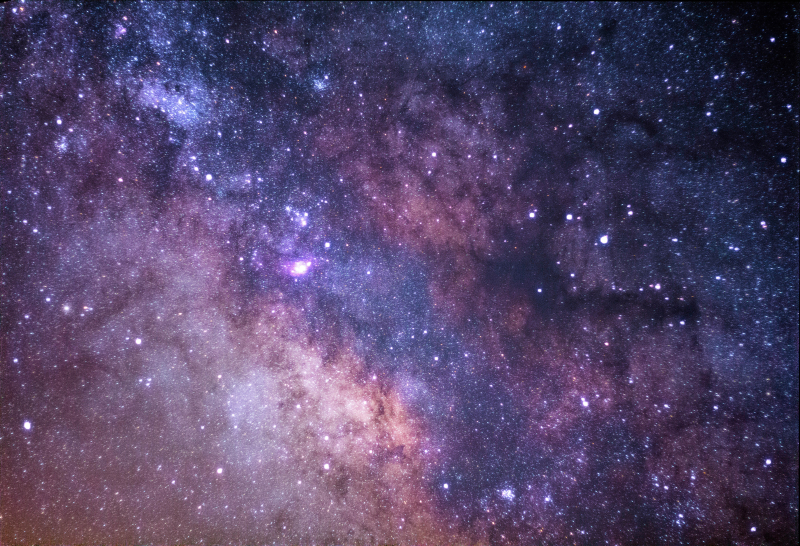
\includegraphics[width=0.3\linewidth]{image-3}
\\[\baselineskip]% adds vertical line spacing
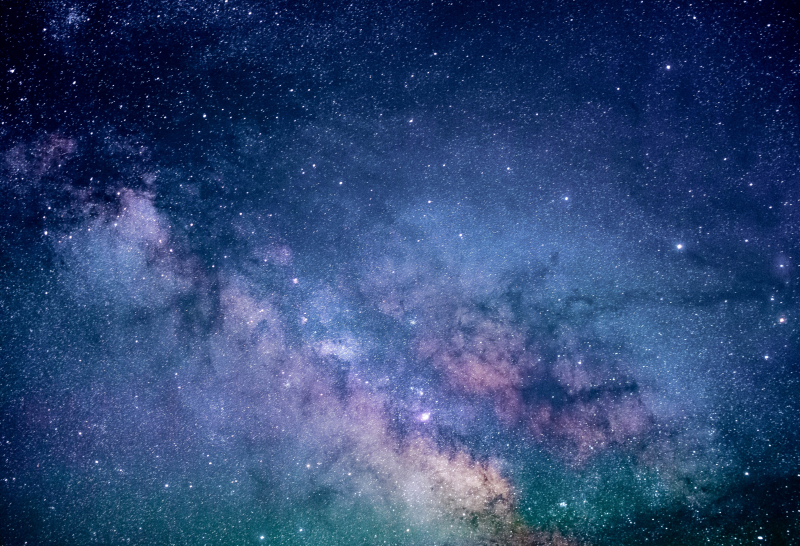
\includegraphics[width=0.3\linewidth]{image-1}
\quad
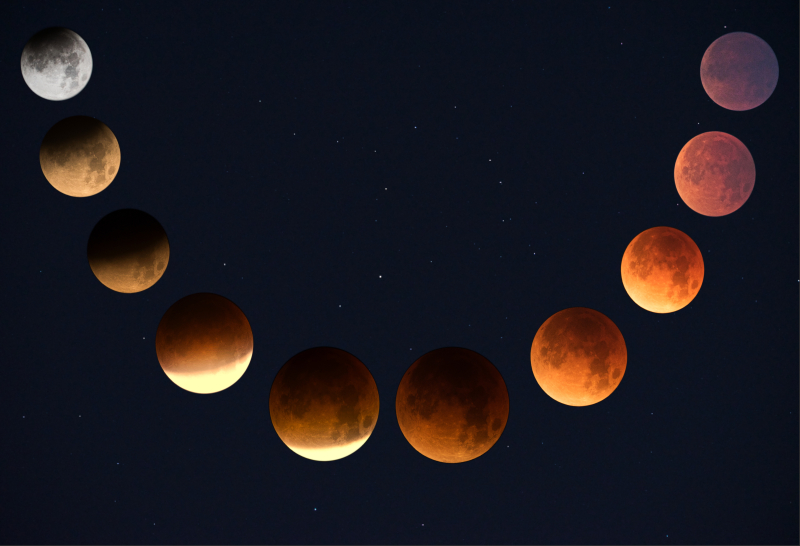
\includegraphics[width=0.3\linewidth]{image-2}
\quad
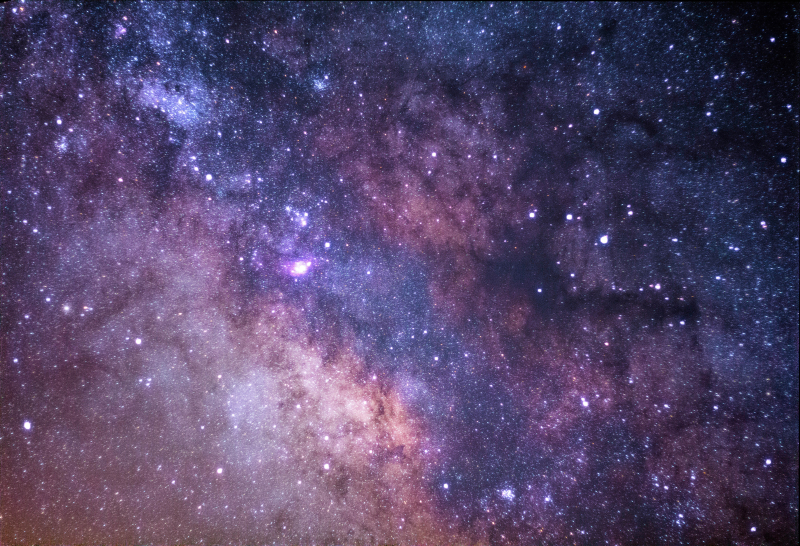
\includegraphics[width=0.3\linewidth]{image-3}

\begin{lstlisting}
  % first column
  \includegraphics[width=0.3\linewidth]{<file-name>}
  \quad % adds horizontal line spacing
  \includegraphics[width=0.3\linewidth]{<file-name>}
  \quad
  \includegraphics[width=0.3\linewidth]{<file-name>}

  \\[\baselineskip] % adds vertical line spacing

  % second column
  \includegraphics[width=0.3\linewidth]{<file-name>}
  \quad
  \includegraphics[width=0.3\linewidth]{<file-name>}
  \quad
  \includegraphics[width=0.3\linewidth]{<file-name>}
\end{lstlisting}

\clearpage
\subsection{Centered Figure}

\begin{figure}[h]
  \centering
  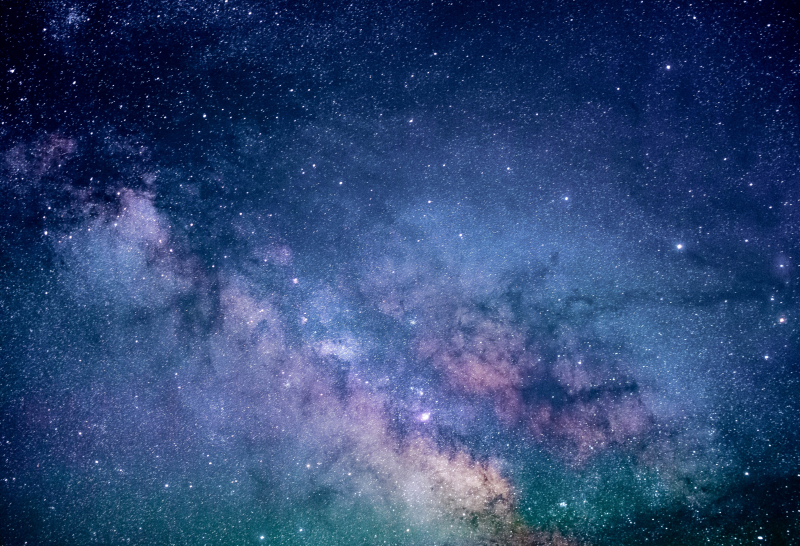
\includegraphics[width=0.5\textwidth]{image-1}
  \caption{This is a centered figure}
  \label{fig:centeredFigure}
\end{figure}

\begin{lstlisting}
  \begin{figure}[h]
    \centering
    \includegraphics[width=0.5\textwidth]{<file-name>}
    \caption{This is a centered figure}
    \label{fig:<yourFigureLabel>}
  \end{figure}
\end{lstlisting}

\clearpage
\subsection{Grid of figures}

\begin{figure}[h]
  \centering
  \begin{subfigure}{0.45\textwidth}
    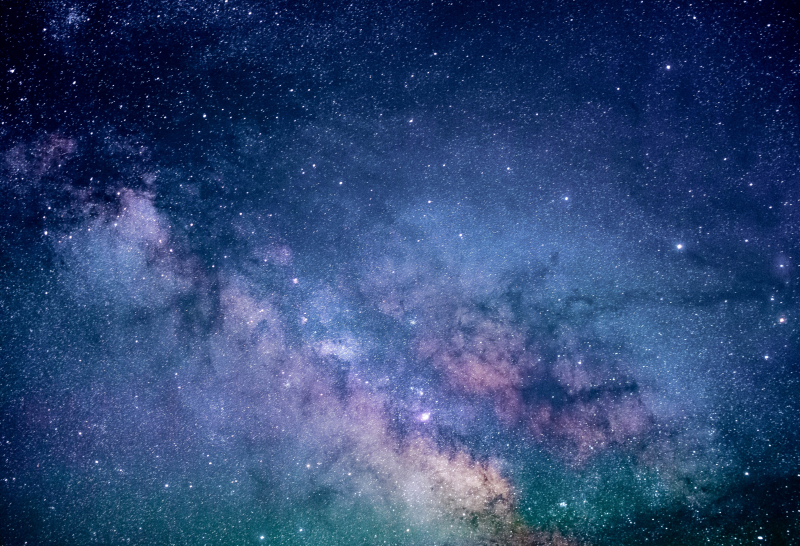
\includegraphics[width=\linewidth]{image-1} 
    \caption{Caption subfigure 1}
    \label{fig:subim1}
  \end{subfigure}%
  \quad
  \begin{subfigure}{0.45\textwidth}
    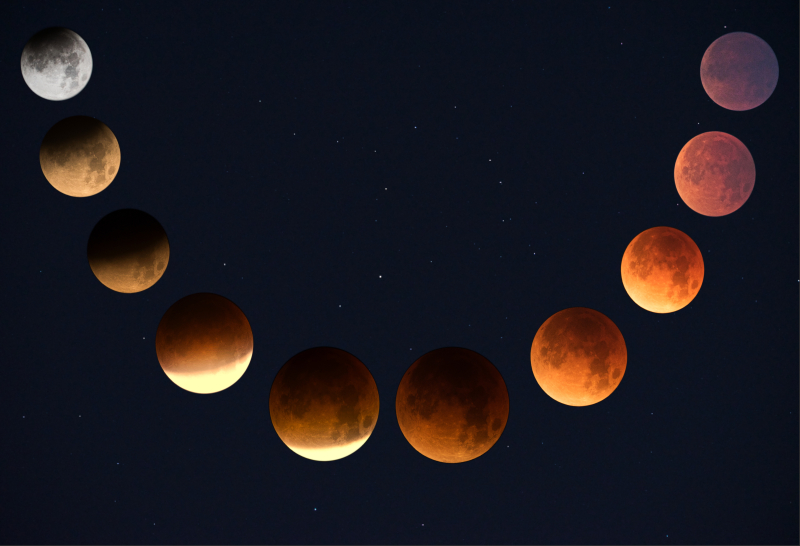
\includegraphics[width=\linewidth]{image-2}
    \caption{Caption subfigure 2}
    \label{fig:subim2}
  \end{subfigure}%
  \caption{This is a grid of figures with two images}
  \label{fig:figuresGrid}
\end{figure}

\begin{lstlisting}
  \begin{figure}[h]
    \centering
    \begin{subfigure}{0.45\textwidth}
      \includegraphics[width=\linewidth]{<file-name>} 
      \caption{Caption subfigure 1}
      \label{fig:<yourSubigureLabel>}
    \end{subfigure}%
    \quad
    \begin{subfigure}{0.45\textwidth}
      \includegraphics[width=\linewidth]{<file-name>}
      \caption{Caption subfigure 2}
      \label{fig:<yourSubigureLabel>}
    \end{subfigure}%
    \caption{This is a grid of figures with two images}
    \label{fig:<yourFigureLabel>}
  \end{figure}
\end{lstlisting}

\subsection{Reference figures}

You can dynamically reference a figure as in \textbf{figure \ref{fig:centeredFigure}} (our centered figure shown above). Also, you can reference the page where the figure currently is, in this case, it would be the page \textbf{\pageref{fig:centeredFigure}}. References will be properly updated if something change with the figure number or page.

\begin{lstlisting}
  % Reference a figure
  \ref{fig:<figureLabel>}

  % Reference a figure page
  \pageref{fig:<figureLabel>}
\end{lstlisting}